%many ways in which the models of previous section would manifest: effects in
%- astrophysics (only way, if dark matter only interacts gravitationally)
%- particle physics (underground, fixed target, and colliders)

The effects of the interactions described in the previous chapter have many consequences, both in astrophysics experiments, where the consequences of gravitational interactions are unavoidable, and in particle physics experiments such as underground DD experiments, fixed target experiments and detectors at particle colliders, where non-gravitational interactions must play a role. 
%why colliders (what is a collider)
%- high energy
%- very well-understood detectors 
%- not able to prove non-interacting particles are invisible particles but
%- discover/study other mediators and other particles in dark sector, not just invisible particles
%why lhc (what is the LHC)
%- interactions may be feeble because because mediator is heavy, or because couplings to SM are small
%- highest energy, able to probe highest energy scales of any collider
%- largest luminosity for hadron-hadron collisions, can reach small couplings
%- complementarity: effective coupling to hadrons required for production in pp collisions, also required for nuclear scattering in DD

To study new types of interactions, collisions of known particles at high energy, observed with very well understood detectors, have been a very successful tool, leading to the discovery of many of the fundamental components of known matter in the SM. %link is completely missing here
Collider experiments alone cannot establish that a newly-discovered invisible particle is invisible particles. But the discovery of such particles at the LHC would open up direct study of their production mechanism, such as observing the SM-invisible particles interaction mediators in other channels, and possible study of additional particle content of the dark sector. %this essentially means we are free from astroparticle uncertainties, more explicit?

The LHC, which presently collides protons at a center-of-mass energy of 13~TeV, is the highest-energy collider in operation.
Since SM--invisible particles interactions may be feeble because of a high mediator mass or small couplings, high energy and large numbers of collisions are needed to probe for them, and the LHC will deliver both in the coming years. 
In the following, we will discuss searches for invisible particles from three LHC experiments, ATLAS, CMS, and LHCb~\cite{ATLAS2008,CMS2008,LHC2008} and briefly touch on some results from previous colliders. %does ALICE search for invisible particles?
Results discussed in this review include up to 36~\ifb of proton-proton data collected up to the end of 2017, a dataset corresponding to more than three times what used for the Higgs discovery and to 1\% of the dataset expected to be collected during the full LHC run including HL-LHC. 

For each type of signature, we will discuss how the relevant searches are done, what some of the challenges are, and how the searches constrain new particle masses and interactions. 
How these constraints affect the potential signals in non-collider searches and the invisible particles abundance are separate issues, that we discuss separately in a later section, where, for example, the LHC bounds on particle properties (couplings, mediator mass, other parameters of the Lagrangian in a particular model) obtained from relativistic collisions are extrapolated to the non-relativistic collisions of invisible particles+nucleons. 

%killed: die fuckers: ATLAS, CMS, and LHCb are well placed to obtain access to high scale and rare process, planning to collect 3/ab by 2035 at the LHC design center-of-mass energy of 14 TeV. 

\begin{marginnote}[]
\entry{Run-1}{First period of LHC running (2010-2012) at 7 and 8 TeV center-of-mass energy, where approximately 20~\ifb of data were collected by ATLAS and CMS.} %this is probably too much information
\entry{Run-2} {Second, ongoing period of LHC running (2015-2018) at 13 TeV center-of-mass energy, planning to collect approximately 100~\ifb of data.}
\entry{HL-LHC} {High-Luminosity LHC running period, planned to start in 2026 to collect 3000~\ifb.}
\end{marginnote}

%transition????
%We start describing searches for invisible particles interacting through SM bosons~\ref{sec:results_ZHSearches}, then move to generic searches for signals of invisible particles with missing transverse momentum and signals of mediators decaying into visible particles~\ref{sec:results_monoXSearches}, outline the searches for complete models with invisible particles candidates in Section~\ref{sec:results_SUSYSearches} and finally conclude with searches for long-lived particles~\ref{sec:results_LLPSearches}. Throughout this chapter
%and in Section~\ref{sec:experimentalChallenges} %CD: removed in favour of sidebars
%we will highlight the experimental challenges and the novel experimental techniques used to overcome them,
%motivated by the strong interest in dark matter searches. 
%We then conclude with searches for long-lived particles within models of invisible particles in
%Section~\ref{sec:results_LLPSearches}. %CD: need to rewrite this sentence, but the idea is: if we hadn't had invisible particles as a motivation motivation we wouldn't have done this difficult stuff. 

\subsection{Searches for invisible particles production mediated by SM-bosons}
\label{sec:results_ZHSearches}

%%%%Z TO INVISIBLE

%- we are sensitive to even lighter neutrinos than 1 MeV wimps
%- we have seen Z decays decay invisibly to light and weakly interacting particles: neutrinos
%-- how have we done that? a visible + MET search (with constraint, at LEP)
%- difference between invisible particles reactions in SM and new physics models: rates 
%- constrain with total Z to invisible
%- results (numbers)

%searching for invisible particles:
%The Z boson has a fuckload of invisible decays

%main background to many other searches for invisible 

%useless info about Z 
%CD only mentioning below because it's like a monophoton
%Simple (but somehow messy) explanation in https://cds.cern.ch/record/1750933/files/CERN-THESIS-2013-330.pdf, Hugo's student
%Hugo did it, unpublished: https://www-cdf.fnal.gov/physics/ewk/2007/ZnunuWidth/
%CDF direct: 466 pm 42
%\textbf{Decays of the Z boson into invisible particles} can be constrained using the invisible Z width. It can be measured directly in Z decays in association with a photon emitted as initial state radiation. Events are selected containing a single photon, missing transverse momentum and no other sizable event activity. This selection is also used for identifying events from possible invisible particles reactions at colliders.
%LEP combined: 503 $\pm$ 16 MeV
%The total Z width has been measured indirectly at LEP~\cite{ALEPH:2005ab} leading to a measurement of the number of light neutrino families compatible with cosmology; if the partial widths of the decays into visible particles are subtracted from the total width, the invisible width can be measured to 499.1 $\pm$ 1.5 MeV~\cite{Patrignani:2016xqp}. 
%The precision of the indirect measurement is better than that of the direct measurement, due to the higher statistics and the relative ease of selection and background subtraction for the visible Z decays. %CD: omitted, no space
%The main systematic uncertainty in this case comes from the theoretical uncertainties in the simulation. CD: Carena seems to think it is an uncertainty on fast simulation
%\begin{marginnote}[]
%Direct and indirect Z width measurements must agree if the decay of the Z to a pair of invisible new particles is to be the main mechanism responsible for the deviation from the SM values. 
%\end{marginnote}%CD: I think this is important to mention in the same sense as the caveats on the s-channel resonances, but it can be omitted
%in this case, an analysis of the mass of the system recoiling against the photon would provide a handle to distinguish between different BSM processes. %CD: omitted because this is possibly too handwavy but how can we summarize 4 pages of Carena in a sentence?
%Carena quantitative: At present, measurements at LEP and CHARM II are capable of constraining the left-handed Z\nu\nu-coupling, 0.45 <~ g_L <~ 0.5,  while the right-handed one is only mildly bounded, |g_R| <= 0.2.

There is already spectacular evidence from high-energy colliders for copious production of low-mass invisible particles mediated by the Z boson: the huge rate of neutrino production. 
The invisible production rate via the Z boson is often the largest background to searches for invisible particles produced through other means, and is therefore important to understand very well.
The rate itself would differ from the predictions of the SM if the Z boson couples to additional invisible particles lighter than about half its mass.
The most precise measurement of the invisible Z width, 499.1 $\pm$ 1.5 MeV~\cite{Patrignani:2016xqp}, has been inferred from the total width at LEP~\cite{ALEPH:2005ab}. This can be used to constrain the parameters of new physics models where the Z decays to new invisible particles, such as Z portals~\cite{Carena:2003aj,Arcadi:2014lta,Escudero:2016gzx}. The coupling between the Z and an invisible Dirac fermion is constrained to be smaller than 2-3\% for invisible particles that are significantly lighter than half the Z mass.
A less-precise direct measurement, also by LEP, uses invisible Z decays in association with a photon emitted as initial state radiation (ISR).
Selected events contains a single photon, missing transverse momentum and little other event activity. This \MET+ISR is a key signature for invisible particle searches at colliders. 
At the LHC, precision measurements of the production and decay of Z bosons can be used to continue testing for the effects of invisible particles in the electroweak sector. 
For example, a measurement from ATLAS of the ratio of cross sections of events containing a jet and \MET, dominated by invisibly-decaying Z bosons, and events where the Z boson decays into an opposite-sign, same flavor dilepton pair, is sensitive to the anomalous production of invisible particles~\cite{Aaboud:2017buf}. 

The Z boson is also key to the invisible decays of the newly-discovered Higgs boson. These Higgs decays contribute to less than 0.1\% of its total decay width in the SM, dominated by the small rate of Higgs decays to a pair of Z bosons that then both decay invisibly. The LHC cannot directly measure the Higgs total width in a model-independent fashion\cite{Dobrescu:2012td}, and its small width to invisible particles in the SM is far below current experimental sensitivity, so an observation of invisibly-decaying Higgs would imply new physics. 
Searches at the LHC either attempt to directly observe the invisible decays of the Higgs boson, via its recoil against visible particles, or compare measurements of the Higgs parameters with their precise theoretical calculations. 
Higgs to invisible LHC searches using Run-1 and Run-2 data employ and combine different Higgs production modes and decays. In all cases, in addition to a requirement of sizable missing transverse momentum, auxiliary visible objects are used to select the events. Decays into invisible particles would reduce the SM Higgs production and decay coupling strengths~\cite{Khachatryan:2016vau,Englert:2011yb,Aad:2015pla}, making precision measurements important to test the presence of new Higgs decays. Combining direct and indirect searches, the most stringent upper limit on the fraction of invisible decays of the Higgs boson is 23\%~\cite{Khachatryan:2016whc,Aad:2015pla}, setting constraints on Higgs portal model couplings of 1-2\‰ for Dirac invisible particles much lighter than half the H mass. 
%For the Higgs boson, the upper limit on the branching fraction to visible and/or invisible non-SM particles only using precision measurements is 34\%

\subsection{Generic searches for invisible particles from BSM mediation}
\label{sec:results_monoXSearches}

Searches for invisible decays of Higgs and Z through Higgs and Z portal models can be seen as tailored instances of more generic searches for BSM mediation of invisible particles. 
The mediator mass plays a role in the LHC phenomenology. The invisible particles are decay products of Z and Higgs, therefore the amount of \MET in the event is limited due to the electroweak 
scale mass of these mediators, and known properties of Higgs and Z bosons are exploited to reject backgrounds. The constraints from these searches are limited to masses of the invisible particles below 40-60 GeV. In order to reach larger mediator and DM masses, a more generic and broader set of searches are employed across a variety of different signatures. 

\begin{textbox}[!h]
\section{Measuring invisible particles: \MET reconstruction}

%10 words per line, 20 lines
%While at lepton colliders the initial center of mass energy is known and 
%can be used as an additional constrain to measure the momentum imbalance due to escaped invisible particles in the final state, measuring missing transverse momentum at hadron colliders
% TJ: Not sure why you make this distinction?
% I tend to think about the lepton collider case as offering
% one extra constraint, i.e. on the total missing *energy*
% but the directional MPT constraint still requires an
% inclusive measurement
Precise measurements throughout each detector systems are crucial to measure \MET in experiments at hadron colliders. This is because the calculation of \vec{\MET} should include all particles in the event.
% regardless of whether they are reconstructed as physics objects (jets, electrons...). 
Contributions that are not attributed to physics objects form the soft component of the \MET~\cite{Aad:2016nrq,CMS-PAS-JME-16-004}. 
One of the main challenges for \MET measurements are excluding contributions other than the hard-scatter process, e.g. from pile-up. 
Searches for invisible particles also need to efficiently reject events with large \MET if the visible energy is due to non-collision background. 

\textbf{Challenge: pile-up in \MET reconstruction.} 
%Momentum contributions from additional proton-proton interactions can have a significant contribution to the overall transverse momentum balance.
In addition to the pile-up suppression techniques applied at the calorimeter level, tracking information can be used to determine whether energy deposits originate from the primary collision vertex. 
The combination of this information is used to remove pile-up both in the physics objects used for \MET calculation and in the overall event energy balance~\cite{CMS-PAS-JME-16-004,ATLAS-CONF-2014-019}. 
%Trigger rates grow exponentially with the number of additional interactions

%[cite: https://cds.cern.ch/record/2205284/files/JME-16-004-pas.pdf, asked Emma and TJ for best reference]
%The lack of tracking information in the trigger system is a limiting factor in selecting events with low \MET at the trigger level, as the rates grow exponentially with the number of additional interactions. 
%from https://twiki.cern.ch/twiki/pub/AtlasPublic/MissingEtTriggerPublicResults/metxs_vs_mu.pdf

\textbf{Challenge: fake \MET rejection.} 
Non-collision backgrounds, such as cosmic rays, beam background and detector noise have a significant contribution to the tails of the \MET spectrum, as shown in Fig.~\ref{fig:fakeMET}
Specific quality cuts, based on the presence of tracks associated to the deposited energy and on energy deposited in the various calorimeter layers are applied to reject these events~\cite{ATLAS-CONF-2015-029}.~\footnote{The number of events passing the jet+\MET analysis selection before these quality cuts is about ten times larger than the SM contribution~\cite{Aaboud:2016tnv}.}. 
\end{textbox}

%Maybe move this to chapter 3

%\subsubsection{Missing transverse momentum}
%\label{sub:MET} 

%Main points:
%\begin{itemize}
%\item The measurement of \MET relies on the precise measurement of all reconstructed physics objects. 
%\item Some description of \MET significance may be needed, but it may also be too academic. 
%\item Fake \MET is rejected using quality cuts.  
%\item Pile-up needs specific techniques because of the soft terms. 
%\item \MET at the trigger level is the driving reason why we can't go lower, see next section.
%\end{itemize}

%from ooutline

%- Mismeasured MET (combining instrumental effects and beam/cosmics background)				
%	- CDF				
%		- beam background: exploit track pointing to jet and calorimeter layers				
%		- QCD: shitty method from Mario (extrapolation changing the veto)				
%	- LHC:				
%		- beam backgrounds: like CDF, more refined				
%			- can have a % of how many events would have been				
%		- QCD: matrix method a la SUSY				
%	- Other backgrounds (diboson, top)				
%		- Small so using MC				
%		- LHC has validation regions				
%			- check ttbar				

%Valerio's talk for relevant plots 
%https://indico.cern.ch/event/466934/contributions/2590281/attachments/1489278/2314178/20170706_EPS_invisible particlesatATLAS.pdf

%MET significance: in VBF CMS search
%For the 8 TeV dataset, an additional requirement is set on an approximate missing transverse energy significance variable S(Emiss) defined as the ratio of Emiss to the square root of the scalar sum of the transverse energy of all PF objects in the event [62]. Selected events are required to satisfy S(Emiss) > 4?GeV.

Many collider searches for invisible particles aim to be model-agnostic. They seek anomalous events consistent with invisible particles being produced, identified by presence of one or a few visible objects recoiling against them, and are designed to detect an excess of \MET over the SM background. 
This has remained the aim of invisible particle searches as center-of-mass energy and dataset size have increased, from LEP to Tevatron to the most recent LHC searches~\cite{Fox:2011fx,Beltran:2010ww,Bai:2010hh}.
Here we discuss these searches, often called 'mono-X' searches, although the radiation of a single object is only the leading process in the reaction~\cite{Haisch:2013ata}. 
We start with the 'jet+\MET' search, which exemplifies many of the challenges and techniques used in other general invisible particle searches.

%We begin this section by describing the LHC searches for missing transverse momentum in association with one or more hadronic jets. The jet+\MET search allows us to illustrate many of the techniques used in invisible particle searches, and it is one of the most powerful to constrain BSM-mediated simplified models of invisible particles. We then move on to outlining searches using different associated objects, and continue with searches for visible mediators that are the consequences of the invisible particles production mechanism. Finally, we compare and discuss the sensitivity of invisible invisible particles and visible mediator searches at the LHC. 

\subsubsection{Searches with jets}

%- searches for invisible particles (where the interaction is mediated by another particle) all have a common denominator in the large Z + (stuff) to invisible SM background
%- for H and Z we know signature is relatively low MET
%- with BSM mediators, we don't: looking in different slices of phase space (different MET regions) with different associated particles (different signal/background ratios and sensitivity to particular operators)

%Can think of searches for H->invisible and Z->invisible as tailored instances of more generic searches where mediator can be whatever the fuck. Invisible signals for masses above 45-60-ish GeV; up to half mediator mass. So: much wider range of the amount of MET is possible. So while the H-invisble searches are tailored to a particular range of mediator masses (90-125 GeV), a more generic set of searches, often termed 'mono-X' searches, are performed to probe this wider variety of signatures found in the BSM mediator models.

One way to approach [this, the goal of model-agnosticism] is to require that the recoiling visible particles are produced by SM processes, not in the dark interaction. ISR meets this criteria. SM bosons are likely to be present in any BSM process, radiated from initial state partons at rates fixed by the SM. Because gluon ISR is far more prevalent than the other forms, the jet+\MET search is important particularly when the details of the dark interaction are unspecified.

Since the presence of highly energetic invisible particles would manifest as an excess of events with a significant \MET, the main observable for this search is the number of events in \MET \textit{signal regions}, either exclusive (in bins of \MET) or inclusive (considering all events above a given \MET threshold). 

To look for signal, the jet+\MET search selects events with a moderate amount of \MET (in the 13 TeV analyses, typically above 200 GeV) and at least one jet with \pt larger than 100-200 GeV in the central region of the detector ($\eta<2.4$). 
%with \pt $>$ 250 GeV (ATLAS) or \pt $>$ 100 GeV (CMS) and \MET $>$ 250 GeV (ATLAS) or \MET $>$ 200 GeV (CMS). 
These \MET and jet \pt thresholds are set in order to achieve a manageable data-taking rate for these events. Selecting events (triggering) in a model-agnostic way is a challenge for models that do not produce a large amount of \MET, because one is forced to assume more about the visible recoil. 

%This selection ensures that all events with these characteristics are recorded by the trigger system for further analysis. Events with lower \MET suffer from higher instrumental and SM backgrounds, which prevents the whole event sample from being recorded due to storage limitations. 

\begin{marginnote}[]
\entry{Trigger}{a detector system that decides which LHC collision events are to be recorded for physics analysis. For a description of the trigger systems of the ATLAS and CMS experiments, see ~\cite{Smith:2016vcs,Aaboud:2016leb,Khachatryan:2016bia}.}
\end{marginnote}

%Searches for invisible particles presents different challenges, depending on the invisible particle mass and boost. If the mediator is heavy, any light invisible particle will receive a boost and appear as an excess in the tails of the SM \MET distribution. If instead the invisible  particle pair originates from a light mediator, of the same mass range as the Higgs boson, it will manifest itself at low \MET. The low \MET suffers from a much higher rate of both instrumental and SM backgrounds.
%As a consequence, it is impossible to record and store all events with a low-\MET for further analysis, since at the data-taking stage (within the \textit{trigger} and data acquisition systems) it is difficult to obtain further handles to discriminate signal and background, and the sensitivity to low-\MET signals is compromised. This challenge will be discussed further for both visible and invisible particle searches in Sec.~\ref{sub:twoBody}.

\begin{marginnote}[]
\entry{Signal region}{a region of phase space for a search that is enriched in signal events. Event counts in this region are used to compare background-only prediction to data in search for discrepancies signaling new physics. 
%For example, a region with a high \MET and no other objects except for the ISR object is a signal region for a \MET+X search.
}
\entry{Control region}{a region of phase space for a search that is signal-free but with characteristics otherwise as close as possible to the signal region. Event counts in this region are used to estimate backgrounds in the signal region. 
%For example, a region requiring no \MET and a process mimicking that of the signal region is a control region for a \MET+X search.
}
\end{marginnote}

%List of backgrounds & cut

From this sample of events, these searches typical further restrict how many hadronic jets and additional visible particles may be present, in order to suppress contributions from SM processes and instrumental backgrounds that can exhibit significant \MET. These requirements reduce the generality of the analysis to an extent but also better isolate signal-like events.
For example, vetoing events with leptons suppresses contributions from W bosons decaying to leptons. 
SM multi-jet processes can exhibit large \MET when one or more jets is mismeasured. Such mismeasurements often result in the \MET pointing in a similar direction as the jet, and this feature is used to reduce this background to about 1\% of the total.
%$\phi$ direction of the missing transverse momentum vector does not align with the direction of the four-momentum of the jets with the highest \pt (leading jets).
%The remaining QCD background estimated from data amounts to less than 1\% of the total background. 
Non-collision events (e.g., intersecting cosmic rays, beam-gas interactions, and calorimeter problems) can also create spurious \MET.
These backgrounds can overwhelm the search, and [much work can go] into designing criteria to identify them. 
Fig.~\ref{fig:fakeMET} are rejected with specific quality criteria.%Sidebar? Textbox?
A restriction on the number of jets above a certain threshold rejects backgrounds from top production. 

The result is a sample consisting mainly of invisible decays of the Z boson (approximately 55-70\% of the total background).
%CMS excludes taus, while ATLAS does not. Too much detail imo. 
%numbers in Livia's talk: https://indico.cern.ch/event/682235/contributions/2817876/attachments/1576792/2490208/invisible particlesWG-2017_V2.pdf and in Francesca's talk:
%https://indico.cern.ch/event/682235/contributions/2817877/attachments/1576793/2490236/171218_atlas_ungaro.pdf
and leptonic decays of the W boson where the lepton is not
reconstructed (approximately 20-35\% of the total background), in association with jets.

\begin{figure}[!htpb]
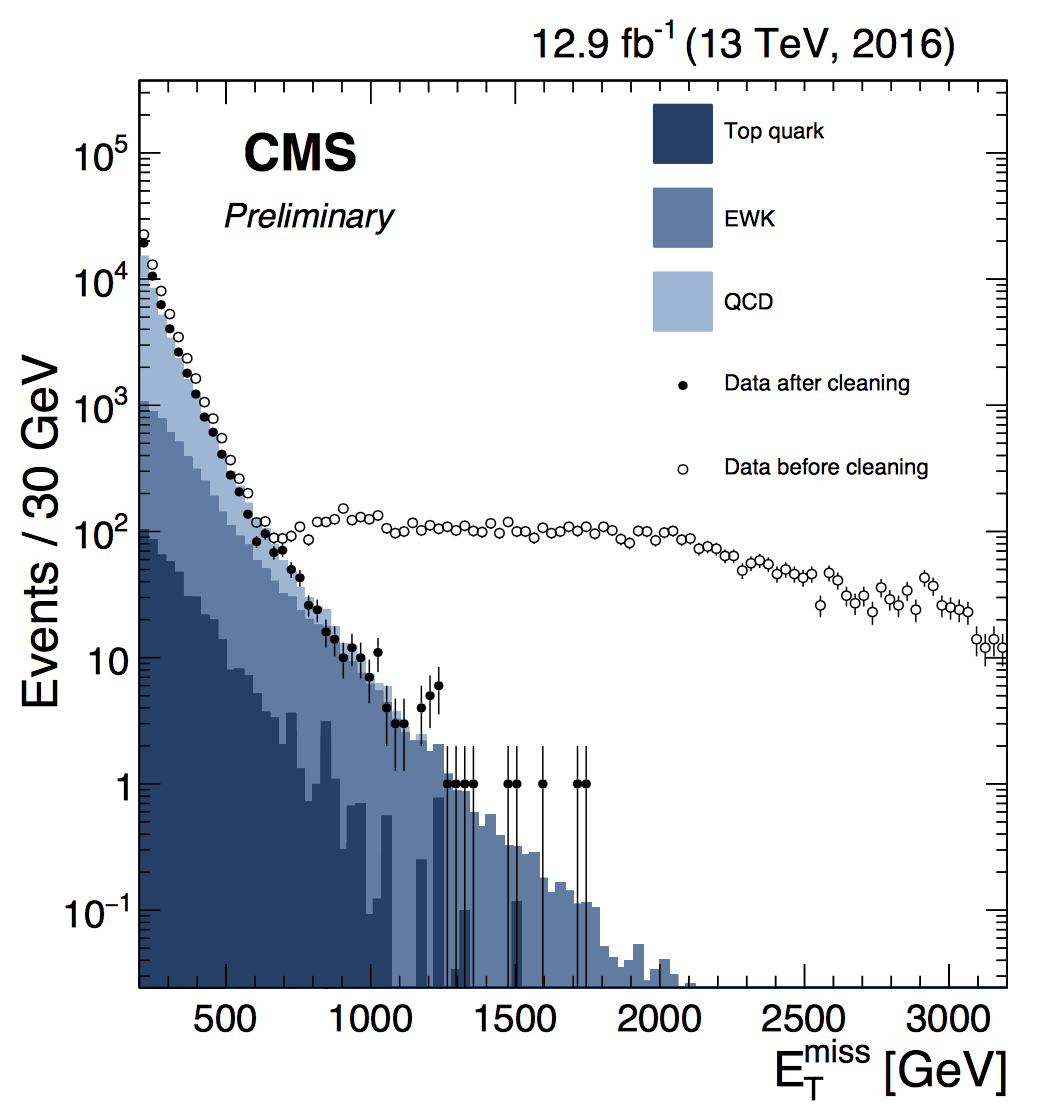
\includegraphics[width=0.5\textwidth]{figures/FakeMETTemp.png}
%Caption from the ATLAS monojet but they only have pT
%https://atlas.web.cern.ch/Atlas/GROUPS/PHYSICS/PAPERS/EXOT-2015-03/
\caption{The \MET distribution of events in data, selected using criteria of high total hadronic energy ad at least two jets with \pt{} $>$ 400 and 200 GeV (open markers), from simulation (filled markers) and
after applying fake \MET rejection criteria.  
%data events passing the [define selection] without any cleaning criteria applied on the leading jet. The Standard Model background indicated in the plots corresponds to the estimates obtained for the analysis signal region, including jet quality requirements. 
%The jet selection inefficiency of the cleaning selection is O(1\%), which is negligible compared to the observed excess in data. 
This demonstrates the necessity of a strong non-collision background suppression for jet+\MET-type analyses. From~\cite{CMS-PAS-JME-16-004}.}
\label{fig:fakeMET}
\end{figure}

%CMS: up to 4 leading jets 
%The CMS analysis also applies specific vetoes for photons and heavy flavour jets, to reject events with photon ISR or containing top quarks. The CMS analysis also includes a signal region targeting hadronic decays of the W and Z bosons using substructure techniques, which is considered separately in the case of ATLAS and will be discussed in Sec.~\ref{subsub:monoV}. 
%Estimating the background
%In order to reduce theoretical and experimental uncertainties on the main backgrounds, 
%
%big picture:
%- need a very precise estimate of the shape
%- calculations of this shape in QCD cannot be done to high enough order to get arbitrarily good precision
%- so predictions from available high order calculations are combined with data in the visible CR to blah.
%- combined means: use Zll as estimate of the shape, compare to MC, and correct for instrumental and other known effects.

High-statistics jet+\MET searches need a very precise estimate of the shape of the background events to be sensitive to signals of feebly interacting particles. 
As an example, the integrated number of signal events with a \MET below 510 GeV amounts to less than 0.03\% of the background~\cite{Sirunyan:2017jix}. 
%>>> 162+130+98+85+65+53+54+41
%688
%>>> 136863+74340+42540+25316+15653+10092+8298+4906
%318008
%>>> 688./318008
%0.002163467585721114
A background estimation solely from simulated events is not precise enough, due to uncertainties on both theory and detector simulation affecting the total cross-sections. 
For this reason, the \MET distribution combines information from both data and the most recent perturbative calculations~\cite{Lindert:2017olm}.
The shape of this distribution is taken from simulation, but its normalization is derived from data in signal-free \textit{control regions} selecting  visible boson+jet processes (W, Z, $\gamma$) 
where the transverse momentum of the visible decay products is subtracted from the total transverse momentum balance to obtain a proxy of the \MET distribution. 
%V+jet processes where the W and Z bosons decay into visible particles ($Z\rightarrow ll, W\rightarrow l\nu+jets$, where $l$ = $e, \mu$). 
%not sure we should say that the bin by bin estimates are used, here it's ambiguous
%The event selection follows that of the signal region, substituting a lepton requirement to the lepton veto in case of vector bosons. 
[Consider adding more info about QCD/QED correction and importance thereof, citing Ellis's paper on UA1 discovery~\cite{Ellis:159861}].
%The estimation of the number of $Z\rightarrow \nu\nu$events from the $\gamma$+jet and  $W\rightarrow l\nu$+jets control region needs a specific treatment due to the difference in the processes. This is particularly important for a consistent treatment of the different processes used in the background estimation and of the main theoretical uncertainties. %CD: how do we call the thing
%The full information on the theoretical and experimental uncertainties and their correlations from this procedure is used in a simultaneous fit to control and signal regions, to determine the overall background estimate in each of the \MET regions considered. 
%and leads to an improvement of 40 to 50% in the search according to PhilHarris and Livia, but I wouldn't add that unreferenced
Backgrounds from top processes in ATLAS are estimated using a dedicated control region with a requirement of a $b-$jet that is included in the fit, while CMS takes this background from simulation. Smaller diboson backgrounds are estimated from simulation. 

%%Experimental uncertainties
The systematic uncertainties on the background estimate for the jet+MET search range from 2 to 7\% (CMS) and 2 to 10\% (ATLAS), depending on the \MET range. The main uncertainties are due to the identification of leptons (CMS) and the understanding of the jet and \MET calibration (ATLAS). 

%- our observable is the rate, then we convert that rate to the parameters of the model: couplings, given masses
%- model-independent as a function of MET cut
%- simplified models and Higgs portal
%  - couplings for different models
%  - Equally sensitive to 

%Model-independent
Having observed no excess over the estimated background, 95\% CL limits are set on the production cross-section of invisible particles, typically spanning from 0.5\pb to 2\fb depending on the \MET threshold~\cite{Aaboud:2017phn}. 
The jet+\MET search can constrain a wide variety of interactions involving invisible particles. Therefore, various approaches have been taken to allow others to easily reinterpret its results. 
As for most LHC searches, the published experimental data from the ATLAS and CMS collaborations is provided on the HEPData platform~\cite{Maguire:2017ypu}. 
Additionally, a simplified likelihood function encapsulating the result~\cite{Collaboration:2242860}, is provided by CMS~\cite{Sirunyan:2017jix}.
%which under certain assumptions approximates the full likelihood using a reduced set of information, 
%and has been used for reinterpretation~\cite{Pobbe:2017wrj}. 
The upper limits on the rates provide bounds on interactions, not necessarily on the masses and other properties of the invisible particles themselves.
ATLAS and CMS jet+\MET results from LHC Run-1, as well as the Tevatron, also constrain EFT models.  
At the LHC Run-2, constraints can be interpreted as limits on the interactions between the mediator and the SM (e.g.\gq) under specific sets of model assumptions. 
For example interactions between (axial-)vector mediators and invisible particles with a coupling \gdm=1 can be constrained up to mediator masses of 1.5--1.9~TeV~\cite{Aaboud:2017phn,Sirunyan:2017jix}. SM couplings of order 0.1 can be constrained for lighter (axial-)vector mediators. 
Jet+\MET searches with the full 2015+2016 Run-2 LHC datasets are beginning to be sensitive to lower-rate interactions with invisible particles mediated by (pseudo-)scalar mediators. 
Limits are also set on colored scalar mediators. For unit couplings and invisible particle masses of up to 100 GeV, the mass of the mediator is constrained to be above 1.7 TeV~\cite{Aaboud:2017phn}. 

\subsubsection{Searches with photons and vector bosons}
\label{subsub:monoV}
%monophoton, monoV

%What we wrote above
%One way to approach the [goal of model-agnosticism] is to require that the recoiling visible particles are produced by SM processes, not in the dark interaction. ISR meets this criteria. SM bosons are likely to be present in any BSM process, radiated from initial state partons at rates fixed by the SM. Because gluon ISR is far more prevalent than the other forms, the jet+\MET search is important particularly when the details of the dark interaction are unspecified.

%- many other searches with ISR+MET
%-- not the higher signal xsec
%-- interesting because they are lower xsec but also higher S/sqrt(B) 
%-- when the details of the dark interaction matter these can be enhanced (VVchichi) 
%-- even for a fixed model, if this is the subdominant channel, different (lower) trigger thresholds. looking for other ISR bosons or additional particles allows lower thresholds and more acceptance for signals 

%i like this part because motivation
Besides the gluon, other particles can constitute the visible-particle recoil against invisible particle production. In the model-agnostic case discussed above, where the recoil arises from ISR, the rates for photon and electroweak boson radiation are much smaller than for gluon radiation. Nevertheless, searches in these other channels can play a complementary role, since they select a smaller and different mix of backgrounds, and are affected by different systematic uncertainties, than the jet+\MET search. Moreover, because of the lower backgrounds, events can be recorded with lower kinematic thresholds than with a jet+\MET search, to probe for interactions resulting in lower MET and visible \pt{}. For example, the lowest \MET value probed by the Z+\MET search, where the Z decays into leptons~\cite{Sirunyan:2017qfc,Aaboud:2017bja}, is around 100 GeV, vs. 
200 GeV for the jet+\MET search~\cite{Sirunyan:2017jix}.

%this tells us about EFT and it's enough
These complementary searches can play a much more powerful role when the recoil arises from the dark interaction itself rather than ISR. In these cases, photon or vector boson recoil~\cite{Birkedal:2004xn,Petriello:2008pu,Carpenter:2012rg,Bell:2012rg}, rather than gluon recoil, may be the dominant signature.

% current song: https://open.spotify.com/track/11CTFD30oBVu5NPSgjLeyi. most of this album sounds like early 80's AC/DC
%i don't know this album enough
%i'm on "love and affection" soon catching up
For these searches, the event selection and the background estimation strategies vary with the type of recoil, and take advantage of the special features of the signal, but generally mirror those of the jet+\MET search, with some relevant differences. 
In the photon+\MET search~\cite{Aaboud:2017dor,CMS-PAS-EXO-16-014}, components of hadronic showers mis-identified as isolated photons are a sizable background that need to be rejected. The searches with ISR bosons decaying hadronically use jet substructure techniques~\cite{Sirunyan:2017jix,Aaboud:2016qgg} to discriminate signal from background, selecting events where the decay products from the high-\pt{} boson are collimated. QCD jets will not present any substructure~\cite{Larkoski:2017jix}, while the decay products of vector bosons grouped into large-radius jets have a typical two-prong pattern from the hadronization of the quark-antiquark pair.

None of these searches presently observes an excess over the estimated background and their results are interpreted as constraints on models of invisible particle production. The searches are not in general as sensitive as the jet+\MET search to models where the visible recoil arises from ISR, because requiring a photon or electroweak boson instead of a jet decreases the background and signal in about the same proportions, but they can be remarkably competitive. For example, after the jet+\MET searches, the photon+\MET searches are the next-to-most powerful.
%, with 95\% CL cross-section limit on invisible particle production constrained to be below 2.5 and 7~\fb depending on the \MET threshold~\cite{Aaboud:2017dor} ranging from 150 to 300 GeV, as opposed to numbers that are not comparable because they are for a different cross section / process.
However, these searches provide the most stringent limits on some models where the boson in question is directly involved in the dark interaction~\cite{Petrov:2013nia,Berlin:2014cfa}.% excluding EFT scales between 150 and 750 GeV for \mdm=100 GeV, assuming the maximal coupling value allowed by perturbativity.

\subsubsection{Search signatures including the Higgs boson}

% what we wrote above Besides the gluon, other particles can constitute the visible-particle recoil against invisible particle production. In the model-agnostic case discussed above, where the recoil arises from ISR, the rates for photon and electroweak boson radiation are much smaller than for gluon radiation

%- old to new: 
%- why we are so keen on doing monohiggs searches:
%
%-- because if DM couples to the Higgs this is the only way to see it 
%--- actually not because monojet in lagrangian too

%- study of higgs properties is a big focus of ATLAS and CMS
%- looking at the higgs in lots of ways
%-how we do Higgs searches: 
%-- like we did before, depending on the decay product, then we stick MET in it and kill backgrounds even further
%-- complementarity between bbar and gammagamma in the same way as before

One can also look for the newly-discovered Higgs boson in the recoil, but due to the heavy mass of the Higgs and the small heavy-flavor content of the proton, the rate of Higgs ISR is insignificant. 
Thus, searches for \MET+Higgs are searches for a dark interaction in which the Higgs is a direct participant, and therefore the interaction is closely tied to the Higgs sector. 
This is a feature of many models that extend the SM scalar sector, as described in Sec.~\cite{sec:BSMMediatorModels}. 

The properties of the Higgs sector are probed at the LHC by many measurements. Dedicated searches for \MET+Higgs select Higgs events with similar selections as the inclusive Higgs measurements, except for the additional requirement of substantial \MET. This additional requirement substantially reduces the backgrounds for the invisible particle searches in the $H \rightarrow \gamma\gamma$~\cite{CMS-PAS-EXO-16-054,Aaboud:2017uak} and $H \rightarrow b\bar{b}$~\cite{Aaboud:2017yqz} decay channels targeted for the analysis of the Run-2 data collected so far. 
%why these channels and not the others
%we could use ZZ but it's not out yet not enough events really even with no ?MET
% other options are: WW and ZZ. these involve lots of additional complications. WW has a lot of different backgrounds, and ZZ is s
%do we say that? no space? i have "due to their relative experimental simplicity and/or high rates"
Searches in other decay channels such as $ZZ, WW$ and $\tau\tau$ with additional \MET are expected to contribute as well, once substantially more data is collected. 

% results / challenges
Searches in the decay channel $H \rightarrow \gamma\gamma$ in association with \MET~\cite{CMS-PAS-EXO-16-054,Aaboud:2017uak} benefit from the high precision and the knowledge of the reconstructed Higgs boson mass. The relatively low backgrounds allow this search to probe \MET as low as 50 GeV~\cite{CMS-PAS-EXO-16-054}. The diphoton invariant mass is fitted in different signal categories, each optimized for different types of signal models. This search is still statistically limited. 
%The SM background is estimated using a fit to the diphoton mass distribution, in events categorized
%according to their missing transverse momentum for CMS (50$<$\MET$<$130 GeV and \MET$>130$ GeV)
%or according to specifications optimised for different signal categories.%this is useless but the analysis is needlessly complicated  
In the search where the Higgs boson decays into two bottom quarks~\cite{Aaboud:2017yqz}
in association with \MET$>$150 GeV, all backgrounds except for the QCD background are estimated using MC simulation and constrained in dedicated control regions. 
This search also employs jet substructure techniques for events with \MET$>$500 GeV, to discriminate boosted Higgs decays from QCD processes. The main systematic uncertainty for the lower \MET signal region is the modelling of the V+jets background, while higher \MET signal region is still statistically limited with the current dataset.

In absence of discrepancies between data and background,
limits are set on the baryonic Higgs benchmark model outlined in
Sec.~\ref{sub:simplifiedModels} with 
\gq=1, \ginvisible particles=1, \ghZprimeZprime/$m_{Z}$=1, \sinthetab=0.3, 
%CMS: mZ'=10-10000 GeV, minvisible particles=1-1000 GeV
%CD: it would be nice to say what this can be reinterpreted to but we have no space
and on a Z'-2HDM models~\footnote{ 
In the case of the Z'-2HDM particles model, CMS and ATLAS set different masses for the 
new Higgs bosons, 
%https://docs.google.com/presentation/d/10R9XJaoMDEhXKhd_Wx9yMXEaPl4uXR8IcmuTeLancvg/edit#slide=id.g1f308da957_0_17
%ATLAS fixes both to 300 GeV, CMS fixes to mA0 
%For the record:
%CMS: A and Z' varied between 300-800 and 600-2500 GeV respectively
%ATLAS: mZ? = 400 to 1400 GeV, mA0 = 200 to 450 GeV
%The masses of the neutral CP-even scalar (H0) and the charged scalars (H�) from Z?-2Hinvisible particles model are set to 300 GeV. The invisible particles mass m? is set to 100 GeV 
%CMS: 
%Two-Higgs-doublet-Z' signals with a pseudoscalar mass of 300 GeV are excluded at 95\% CL for Z' masses below 900 GeV
%Baryonic Z' models with a invisible particles mass of 1 GeV are excluded at 95% CL for Z' masses below 800 GeV
so the constraints are not yet directly comparable.}. Higgs+\MET and Z+\MET searches are also sensitive to extensions of the scalar sector including two Higgs doublets and a scalar or pseudoscalar mediator~\cite{Bauer:2017ota,Ipek:2014gua,No:2015xqa,Goncalves:2016iyg,Bell:2016ekl}, although this is not an interpretation of ATLAS and CMS searches so far. 

% with $tan\beta$=1, \gZPrime=0.8 and \mdm=100 GeV

%this is a dump, too long? i can't quite see how to make parallels between the two searches as they are really different


i like this commercial def leppard album
adrenalize
KEY CHANGE
babythatistrue
%Events are categorized according to their missing transverse momentum for CMS (50$<$\MET$<$130 GeV and \MET$>130$ GeV)
%or according to specifications optimized for different signal categories. 



and the ability to probe low \MET 



thresholds compared to other Higgs decay channel as the trigger rates are low. 
The main uncertainty for the $H \rightarrow \gamma\gamma$ searches using the 2015+2016
LHC Run-2 dataset is statistical. 


% see below, need to prune a lot

what are commonalities and differences in the two mono-H channels
how are they differently analyzed from the others
- H->bb and H->gamgam
- known higgs mass
- looking for peak on smooth background
they are completely different 
we could introduce here the fit to smooth distribution

https://open.spotify.com/track/54lmjC4P1kWvN38LgmBd1a?si=mwHA-NPoQCq3hposUjPgLQ
have you ever tried so hard that the words blah
i gotta heavy babe



ok problem: the ATLAS search is so complicated because of the overoptimization for the mandala boson that we can't really get away without the NNNNNN signal categories 
CMS has an easier way of doign thigns

%https://open.spotify.com/track/1habYP727aDxAH11D9JmuJ?si=UpFPdECNToGySuEPCeEbcg
%obvious chords i like it

- results 
-- there are so many models we don't really want to talk about them (also ATLAS and CMS use different parameters and it's awkward)
-- 2HDM??????????
-- the mandala boson is shit public statement?




%CD: I kinda want to say this but we have no space so why bother
%the mandala boson is shit, misguided attempts at combining Higgs discovery with every other excess


%where do we use the assumption of this dark interaction in the kinematics? does this mean stuff is less model independent? 
%yesthis would be a nice transition to SUSY after but then i would move the bbar+MET above this, not su.re why  oikt's below


wait though
where do we put dijets then? logically

maybe we have 1) searches with MET 2) searches without MET
or 
se
archseuss yss
s

susy -> more powerful searches when you see other consequences of the interaction -> dijets
SUSY = MET
MET = SUSY


yes that is another chapter altogether
dijet after SUSY?
not sure
people forgot monojet by then

right now outline is:

- searches for H and Z portals
- generic searches with MET
-- MET+jet
-- MET+V
(first transition about what we know about the interaction helps us, but still linked to earlier because no assumption on the interaction, only about the production)
-- MET+HF
(second transition about what we know about the interaction helps us)
-- MET+H
- generic searches without MET (dijet goes here)
- SUSY searches
- LLP searches


(aside: olegplan for whitepaper will need corrections, they are less sensitive than monoZ at not-particle-level)
--- here we don't use monojet techniques, we do shittons of fits that i don't really want to talk about

%monoH, H to invisible detailed earlier on

\subsubsection{Searches with heavy-flavor quarks}
%ttbar+MET
%reinterpretation of SUSY

Generic searches employing one single additional object produced in association with \MET
are powerful tools to probe simple models of invisible particles. More complex models, however, bring 
more handles for discovery: steps in this direction can be taken with searches using 
scalar and pseudoscalar models as benchmarks, where information about the production mechanism 
(e.g. the mediator is produced in association with two heavy flavor quark, complementing the
gluon-fusion production mode of the \MET+jet searches) is exploited in 
the search strategy. 

The searches in~\cite{Aaboud:2017rzf,CMS-PAS-EXO-16-051}
are optimized for invisible particles scalar and pseudoscalar mediators
selecting events in the semileptonic and fully hadronic top quark decay channels,
as well as events containing one or two bottom quarks, in association with \MET. 
The dominant backgrounds in~\cite{Aaboud:2017rzf} are estimated separately
using MC in each of the signal regions,
and their normalization constrained using control regions in a simultaneous fit.
The main uncertainties for these searches are, depending on the signal region, 
theoretical and MC simulation related uncertainties, jet energy scale and resolution. 
and uncertainties related to the identification of heavy flavor quarks. 
Signatures including \MET and two heavy flavor quarks are similar to 
signatures of third generation quark superpartners, leading to dedicated
invisible particles signal regions being included in SUSY searches or used
for reinterpretation~\cite{Aaboud:2017aeu,CMS-PAS-SUS-17-001}. 
In SUSY-like searches, the dominant $t\bar{t}$ backgrounds
are heavily suppressed using variables that combine visible and invisible
mass~\cite{Lester:1999tx} targeting the model sought. 
This step uses information that is model-dependent,
but increases the sensitivity to specific processes. The remaining
small backgrounds are estimated using simulation. 

The sensitivity of searches of \MET associated to top quarks
is comparable for the two strategies. 
For a choice of \minvisible particles=1 GeV, pseudoscalar mediator masses of 10-50
GeV~\cite{AAaboud:2017aeu} and scalar mediator masses up to 100
GeV~\cite{CMS-PAS-SUS-17-001} are excluded. 
%CD: it would be nice to find out why this difference in sensitivity? 
The increased LHC dataset 
will allow these searches to be sensitive for other invisible particles masses. 
%CD: this sentence is shit but i'm tired
Signatures with $b\bar{b}$ pairs are less sensitive to
scalar and pseudoscalar mediators that do not explicitly
privilege bottom quarks. Mediator masses for the b-flavored colored scalar 
model discussed in~\cite{Agrawal:2014una} are excluded up to 1.1 TeV
for \minvisible particles=35 GeV. 

%Not spending more than one sentence on monotop, is that ok?
Other searches in the heavy flavor+\MET category are those only
including only one top or bottom quark
(also called mono-top or mono-bottom searches)~\cite{CMS-PAS-EXO-16-051, Aad:2014wza},
and place constraints on models that include singly-produced invisible particles candidates
through flavor-changing neutral currents, described in~\cite{Boucheneb:2014wza}. 

%The main backgrounds for these searches are single top or misidentified $t\bar{t}$ processes. 
%The search where the top quark decays hadronically
%employs substructure techniques to tag the boosted top quark decays.  
%These searches place constraints on models of invisible particles (resonant, non-resonant). 

\subsubsection{Two-body mediator searches}
\label{sub:twoBody}
%Dijet and dilepton
%Mention TLA


\subsubsection{Consequences of neutral-mediated models: visible decays}
\label{sec:MediatorSearches}

JUNK

As mentioned in the earlier section, if the mediator particle can produced from from interactions of
quarks and gluons, it may also decay in quarks and gluons. 
For this reason, it is worthwhile that collider experiments not only search for
the invisible invisible particles particles, but also probe directly the interaction between Standard Model and 
invisible particles particles by searching for the visible decays of the particles that mediate it, as shown 
in Figure~\ref{fig:monoX} (c) and summarized in e.g. Refs.~\cite{Liew:2016oon,Fairbairn:2016iuf}. 

%CD cite the following
%Coupling--mass mapping of di-jet peak searches, 10.1103/PhysRevD.88.035021 ok
%Searches for Dijet Resonances at Hadron Colliders, 10.1142/S0217751X11054905 in the experimental part, i would say
%Searching for Low Mass Dark Portal at the LHC, 10.1016/j.dark.2013.03.002 ok
%Constraining Dark Sectors with Monojets and Dijets, 10.1007/JHEP07(2015)089 ok
%Constraints on Z? models from LHC dijet searches and implications for invisible particles - https://arxiv.org/pdf/1605.07940.pdf -> ok

At the LHC, such mediators would be produced by colliding two partons,
and thus one could studying them via their decays to jets. 
%Dijet searches are sensitive to vector and axial vector invisible particles mediators decaying 
%exclusively to jets with couplings that would satisfy relic density constraints~\cite{Chala:2015ama}.
%but also to new, unknown particles that might be created when crossing 
%the threshold of a new energy scale. 

%it is not possible to claim a discovery of invisible particles mediators at the LHC without
%corresponding excesses in invisible channels and non-collider experiments. 

Nevertheless, these benchmark models have motivated novel search techniques
to look for low-coupling, low-mass resonances below the TeV scale that would
have otherwise not been explored in early Run-2 data due to experimental difficulties~\cite{An:2012ue,Dobrescu:2013coa}. 


%All citations from invisible particlesF, probably want to save citations for later
%They are sometimes necessary in order to construct a consistent theory, for example in minimal completions of the axial-vector model [11, 12] or in models with extended Higgs sectors [13, 14]. They often appear in anomaly-free spin-1 mediator models [15], see also Section 3.3.2 of [7]. They may also be induced through radiative corrections (e.g. through quark loops that lead to Z??Z mixing). The near-ubiquity of lepton couplings in full theories motivates including them when searching for visibly-decaying spin-1 mediators.

%Generic resonance searches sensitive to a broad range of theoretical models 
%are already the focus of LHC. 

END JUNK

Decays into pairs of SM particles are an inevitable consequences of models where
invisible particles mediators are exchanged in the $s-$channel and have a SM coupling. 
This possibility to probe the SM-invisible particles interaction through the visible 
decays of mediator is a unique feature of collider experiments
%and can be exploited for dark boson models as well? 
and one that they are well-prepared for, with a wealth of generic searches for
two-body resonances (see e.g.~\cite{Harris:2011bh}).
In the following, we will describe two of the most general examples,
the searches for dijet and dilepton resonances, their challenges and the implication of their results
for models of SM-invisible particles mediation. % including a Z'-like mediator. 

%Describe dijet search
\textbf{Searches for dijet resonances} exploit the smoothness of the falling QCD background
to derive their background directly from a fit to data. This minimizes modelling
and theoretical uncertainties. Localized excesses are sought atop %woo atop!
the fitted background estimation~\cite{Aaboud:2017yvp,CMS-PAS-EXO-16-056}. 
%Where dijet lose sensitivity: wide signals, angular 
If the resonance is wider than 15\%, as in the case of 
vector and axial vector mediator models with couplings roughly above \gq$>$0.5~\footnote{This value
assumes that the new particle can decay only to quarks and invisible particles particles, with \ginvisible particles=1.0 and \minvisible particles=1 GeV.}, 
the fitted background estimation will be biased by the presence of signal. 
In this case, the \textbf{scattering angle of dijet events} can be exploited as a discriminating variable, 
since the QCD background is dominated by $t-$channel processes that privilege
large angular separations between the two jets, as opposed to signals with an isotropic angular distribution
in the center-of-mass frame that translates to the presence of more central jets in the
detector~\cite{CMS-PAS-EXO-16-046,Aaboud:2017yvp}.  
%$s-$channel scattering processes are more in the center-of-mass frame
%are not 
%in case of wide resonances, 
%and below the trigger thresholds .  

%Where dijets lose sensitivity: low-mass 
Standard LHC dijet searches lose sensitivity at masses below the TeV, where the high QCD
rates force the experiments to randomly discard a large fraction of background and
signal events alike (see sidebar). %sidecar, not sure how to call this but we can ask for help
An example of such a technique is recording only \textbf{partial event information} for later analysis directly 
from the trigger system (called Data Scouting in CMS~\cite{CMS-PAS-EXO-16-056},
Trigger-object Level Analysis in ATLAS~\cite{Aaboud:2016leb}, Turbo Stream in LHCb~\cite{Aaij:2016rxn}),
to overcome the data storage constraints. 
Dijet resonance searches that use this technique~\cite{CMS-PAS-EXO-16-056,ATLAS:2016xiv}
can record the full rate of dijet events to much lower dijet invariant masses than the standard dijet
searches, but have to overcome a number of challenges that go beyond
a seemingly simple search. The first challenge is demonstrating that the
performance of the physics objects reconstructed at the trigger level is sufficiently good
to perform a physics analysis and not just take a decision on whether to keep the event.
Secondly, the extremely large background rates (above 10$^5$ events/GeV) grant
a sufficient statistical precision to observe signals of the order of a few thousand events,
but also per mille-level detector and SM contamination effects. 
An alternative data-taking strategy is to require a \textbf{high-\pt{} ISR object} to trigger
on the event and reduce the QCD background, but the sensitivity is reduced by this requirement with
respect to selecting the leading order dijet process. The ISR object can be either a jet and a photon,
and it recoils against a dijet pair. The dijet pair can be either resolved~\cite{ATLAS:2016bvn} or
collimated and reconstructed within a large-radius jet tagged with substructure techniques~\cite{Sirunyan:2017nvi},
depending on the ratio between mass and transverse momentum of the resonance
that boost the decay products. If the mediator particle decays democratically to
different quark flavours or preferentially into heavy flavour quarks (as in the case for a scalar mediator),
searching for \textbf{$b\bar{b}$ or $t\bar{t}$ resonances}~\cite{lowMassDiB,CMS-PAS-HIG-16-025} 
can overcome the data taking constraints 
at masses above roughly 500 GeV and have a sensitivity comparable to inclusive 
dijet searches for vector and axial vector mediators. An interesting feature of 
scalar and pseudoscalar particles decaying to $t\bar{t}$ 
is their interference with SM $gg \rightarrow t\bar{t}$ production~\cite{Djouadi:2016ack}
that has to be explicitly accounted for when estimating the background for these searches
~\cite{Aaboud:2017hnm}. 

TODO: add coupling-mass summary plot for ATLAS
%TLA and challenges, point to sidebar

%Sidebar (50 words minimum, 200 words maximum) briefly discussing a fascinating adjacent topic; 
%insert below Literature Cited section, but indicate near which section in text the sidebar should be typeset
%Consider swapping with the ERC text below?
\begin{textbox}[!h]
\section{Selection of events at the detector level (trigger)}
%Trying to approximate 10 words per line
%Notes for improvement: 
%this is too long, needs sharpening. 
% the points i want to make are:
% higher thresholds are bad for mediator searches and also in general -> go TLA
% pileup increases MET thresholds -> get track info at the trigger level
%it needs a much clearer motivation: model X gives low mass. 
%probably that needs done in the text because space constraints, but then why using this box-thing (other than tidying things up)? 
The LHC collides protons every 25 $\mathrm{ns}$, producing 40 billion 
of events per second at nominal conditions. This amount of data cannot be 
recorded in its entirety, and not all events are interesting
for the experiments' physics programmes. %programmes or programs?
A trigger system is used to decide whether an event is selected for further analysis. 
Its first level is realized in hardware and only uses
partial detector information for fast decisions in a time of
the order of $\mathrm{\mu s}$, while its second level is software-based
and uses more refined algorithms and information to make a
decision in $\mathrm{ms}$. 

\textbf{Challenge: triggering on low-\pt objects}
Since the rates of SM physics processes decrease
with the transverse momentum of the objects involved, and processes
with a high momentum transfer have a higher chance of containing
interesting features or new particles, the trigger system records
events above a certain threshold e.g. in leading jet \pt or in event \MET. 
Only a fraction of events that do not satisfy these thresholds is recorded. 
Searches for signals with high-rate backgrounds and 
MET or jet \pt below these thresholds are 
therefore penalized unless novel
%not novel anymore?
data recording techniques, such as only recording partial event information 
needed for the search, are employed.

\textbf{Challenge: \textit{pile-up} in trigger} Simultaneous proton-proton interactions occurring within the detector
readout time cannot be completely disentangled from the hard process
of interest, especially if reconstructing the collision vertex
is not possible at the trigger level due to CPU constraints. 
This \textit{pile-up} increases the likelihood of passing 
the minimum threshold to record events, especially in the \MET triggers.
For this reason, the increase in the LHC instantaneous luminosity by virtue
of increasing the number of simultaneous
collisions leads to increases in the trigger thresholds to
keep manageable event recording rates. Reconstruction algorithms that suppress
the effects of pile-up can be employed by ATLAS and CMS directly at the trigger level,
using information on the objects and energy density within the event~\cite{CMS:2014ata,ATLAS-CONF-2014-019}. 
In future LHC runs, track information to disentangle the provenance of the 
energy deposits from the collision vertex will be available for
ATLAS and CMS from dedicated hardware systems (see e.g. Refs.~\cite{Shochet:2013gaw,1748-0221-6-12-C12065}). 
\end{textbox}


%Describe dilepton and remind of why we want to include dilepton
Searches for new particles decaying in opposite-sign, same-flavor lepton pairs~\cite{Aaboud:2017buh,Khachatryan:2016zqb} can also be interpreted in terms of the simplified models of invisible particles, 
if the mediator particle has sizable couplings to leptons. Although lepton couplings
are not mandated by the quark-antiquark production at hadron colliders as dijet couplings are, 
lepton couplings feature in a variety of models that can embed
the simplified models of invisible particles used as benchmark for LHC searches. %this sentence repeats the one in Sec.2. 

The main backgrounds for the dilepton searches in electron and muon final states 
arise from Drell-Yan processes, and are estimated using simulation corrected for NNLO effects and normalized to the Z boson peak event yield in data. 
%ATLAS. too much detail
%The background prediction is smoothed using functional fits where the number of simulated events is not representative of the data statistics. 
Reducible backgrounds where other objects are mismeasured as leptons are estimated using data. The main uncertainties on the background estimation are of theoretical nature, for the entire invariant mass range. 

%List constraints from both searches with two coupling options
%The CMS analysis also scans the coupling-mass plane by fixing the ratio between \minvisible particles and \mmed to ensure perturbativity 
%CMS sentence: Quark couplings down to 0.05 for mediator masses at 50 GeV are excluded for the spin- 1 simplified models as shown in Fig. 12. 
The same constraints from dijet and dilepton searches apply to both vector and axial vector mediators:
the LHC phenomenology (rates and kinematics) is the same for both. Searches for visible mediator decays 
are sensitive to masses as low as 50 GeV (boosted dijet) and constrain SM-invisible particles couplings \gq as low as 
0.05 at 60 GeV. Jets from the mediator decay start being spatially separated above mediator masses of 250-300 GeV, 
and that is where the resolved dijet+ISR topology takes over in terms of sensitivity, with the $\gamma$ ISR + dijet channel
constraining \gq$>$0.15-0.2 up to 350 GeV, where the jet ISR + dijet channel is not limited by
trigger thresholds anymore and is more sensitive due to the higher gluon radiation rates.
Searches with jets at the trigger level are the most sensitive to low-mass mediators where available,
excluding simplified models with \gq as low as 0.05 starting from 400 GeV. 
Standard dijet searches constrain models with invisible particles mediators up to 3 TeV.  
%but lose sensitivity to lower couplings where they start to be statistically limited. 
Dilepton searches are more sensitive than dijet searches in case of equal couplings
of the mediator to leptons and jets, due to the much reduced backgrounds. ATLAS and CMS searches
with the 2015+2016 dataset probe signal masses starting from 150 and 400 GeV respectively.  
%what is the minimum coupling by dilepton searches? not sure this is easy to do without reinterpretation

%Mention LianTao's paper where baryonic / 2Hinvisible particles monoHiggs is also constrained. 
%Mention results of other searches: ttbar resonances for pseudoscalar with interference, Higgs-like scalars (CMS boosted) 

\subsubsection{Comparison of sensitivity of visible and invisible LHC searches}
\label{sub:comparisonVisibleInvisible}

JUNK: The parameter values used as benchmarks (e.g. couplings) have been selected considering the sensitivity of early Run-2 searches, precision constraints and general simplicity arguments. As described more in detail in Section~\ref{sub:comparisonVisibleInvisible}, results are given in the \mdm particles, \mmed  plane fixing the couplings to \gq=0.25 and \gdm particles=1.0 for vector and axial vector mediated models, \gq=\gdm particles=1.0 for scalar and pseudoscalar models and \gdm particlesq=1.0 for colored scalar models. The simplified models employed by the experimental collaborations are known at NLO~\cite{Neubert:2015fka,Haisch:2013ata,Backovic:2015soa}. 


It is important to note that generic searches for new two-body resonances
are by design sensitive to a broad range of theoretical benchmarks, 
and as such they alone can offer little information on 
whether a discovery would imply in terms of invisible particles mediators.
In absence of a signal and within a specific model scenario,
searches for mediator particle with visible decays
provide constraints that are complementary to those of searches
for invisible particles particles, in particular in the off-shell region 2\minvisible particles $>$ \mmed where the mediator
cannot decay to invisible particles directly but can still decay into much lighter SM particles
such as leptons and quarks. 
The relative sensitivity of the two kinds of searches
is a model- and parameter-dependent statement: for $s-$channel simplified models
searches for invisible particles particles only dominate if the coupling to invisible particles is much larger
than the coupling to quarks, and even then reducing \gq reduces the LHC production
cross-section and therefore the overall sensitivity of \MET+X searches. 
One advantage of searches for invisible particles is their sensitivity to models with
very light mediators ($<$50 GeV), since the reach of dijet and dilepton searches to low-mass
resonances is still ultimately limited by data taking constraints. 

%Mention why we plot things in the mass-mass plane. 
A sketch of the comparison of the sensitivity of searches for visible decays of vector and axial vector mediator models, and invisible invisible particles particles 
in the \minvisible particles vs \mmed plane is shown in Fig.~\ref{fig:sensitivityComparison}, fixing the couplings. The choice of plane and the scenarios chosen follow the choices of the Dark Matter Working Group~\cite{Albert:2017onk}, to illustrate the complementarity of different LHC searches for $s-$channel-mediated model of invisible particles and to convey the message that the sensitivity of LHC searches to simplified models of invisible particles depends both on model choice and parameter choice. 
%Mention why mass-mass? Because on-shell/off-shell regions clearly spelled out

The topmost left-hand side figure shows a leptophobic vector mediator with \gl=0, \ginvisible particles=1.0 and \gq=0.25, where dijet searches for visible decays of the mediator constrain both on-shell and off-shell region but are limited by data-taking constraints at masses above roughly 50 GeV, where \MET+X searches take over in the on-shell region. An equivalent picture is drawn for the vector mediator, in the top right plot. The bottom right plot shows the case of an axial vector mediator with reduced quark couplings and equal lepton couplings (\gq=\gl=0.1 and \ginvisible particles=1.0), where it can be seen that searches for dilepton resonances cover a larger range of parameter space with respect to dijet resonances but are still limited at low mediator masses; the region constrained by from \MET+jet searches extends to lower invisible particles and mediator masses with respect to the case of the model with \gq=0.25 due to the reduced production rate. The third panel in the bottom left shows the scenario of a vector mediator where lepton couplings are reduced with respect to quark couplings (\gq=0.1, \gl=0.01, \ginvisible particles=1.0), where the range of all regions constrained by visible mediator decay searches is considerably reduced with respect to the scenarios with larger couplings. 

%TODO: make more visible, limit to 2 plots
\begin{figure}[!htpb]
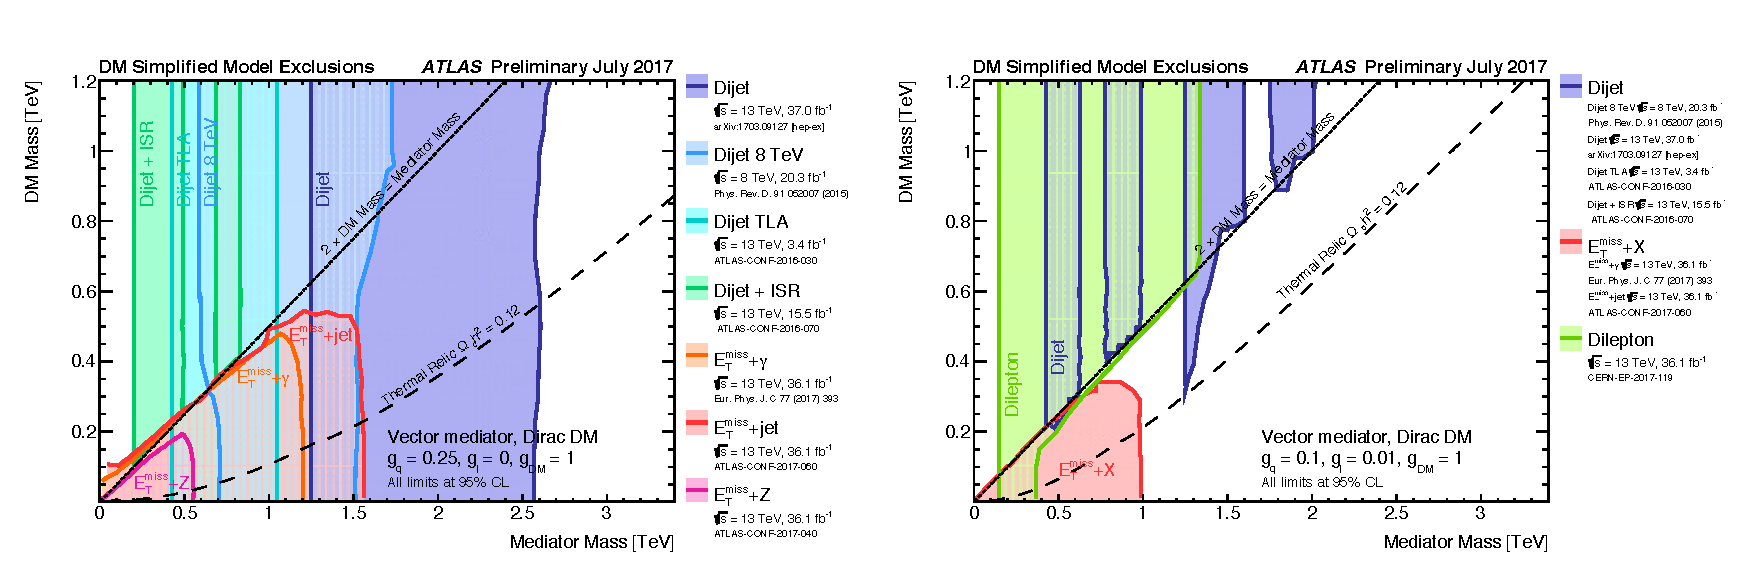
\includegraphics[width=\textwidth]{figures/SummaryPlotsMassMass.pdf}\caption{
Regions in a dark matter mass-mediator mass plane excluded at 95\% CL by a selection of ATLAS dark matter searches, for a vector mediator benchmark model with varying coupling scenarios. Top plots: \gq=0.25, \gl=0.0, \ginvisible particles=1.0, axial vector (left, separate search constraints) and vector mediator (right, combined search constraints), highlighting the sensitivity of visible searches in this scenario and the near-equivalence of the vector and axial vector as benchmark models for LHC searches. Bottom plots: \gq=0.1, \gl=0.1, \ginvisible particles=1.0 for an axial vector mediator (left) and \gq=0.1, \gl=0.01, \ginvisible particles=1.0 for a vector mediator (right), highlighting the sensitivity of the lepton searches and its dependence on the chosen coupling value. Dashed curves labeled "thermal relic" indicate combinations of dark matter and mediator mass that are consistent with a dark matter density of $\omega_c = 0.12 h^2$ and a standard thermal history, as computed in MadDM particles~\cite{Backovic:2015cra}. The dotted curve indicates the kinematic threshold where the mediator can decay on-shell into dark matter. }
%\ginvisible particles=1.0  \gq=0.25universal to all flavors, and a lepton coupling gl set to zero. This choice of couplings corresponds to the "V1" scenario in arXiv:1703.05703. Leptonic decays are absent at tree level. The results use 13 TeV data except for Phys. Rev. D91 052007 (2015). The exclusions from the ATLAS dijet searches are derived from the limits provided on Gaussian-shaped resonances following the procedure recommended by ATLAS in Appendix A of Phys. Rev. D91 052007 (2015) and in arXiv:1703.09127. Small fluctuations in the contour are a product of the dijet reinterpretation scheme. 
%To the left of the curve, annihilation processes described by the simplified model deplete ?c below 0.12 h2. A dotted curve indicates the kinematic threshold where the mediator can decay on-shell into dark matter. The exclusion regions, relic density contours, and unitarity curve are not applicable to other choices of coupling values or model.
\label{fig:sensitivityComparison}
\end{figure}

%CD: if we want coupling-mass, we could show the plots in the figs dir: SummaryPlotsCouplingMass.pdf

%In case sample figure with different scenarios as an example
%\begin{figure}[!htpb]
%\includegraphics[width=\textwidth]{figures/invisible particlesSummary.png}
%\caption{Illustrative examples of the comparison of the sensitivity of searches for visible and invisible mediators in the \minvisible particles-\mmed plane, for different coupling scenarios. No actual data has been used, but experimental observations have been used as inspiration for the figure. From~\cite{AnotherWikipedia}.}
%\label{fig:sensitivityComparison}
%\end{figure}

%It would be nice to make tables of lowest mediator/invisible particles searches+refs for 100 GeV invisible particles mass,
%as a poor-person approximation of a summary plot we can't make because ATLAS data not public. 

%%%SUMMARY TABLE FOR MONOX SEARCHES: descoped, unless we just want a list of references of all the searches which may be useful but obsoletes early
%\begin{table}[h]
\tabcolsep7.5pt
\caption{Summary of searches for BSM mediators at the LHC}
\label{tab:BSMSearchesSummary}
\begin{center}
\begin{tabular}{@{}l|c|c|c|c@{}}
\hline
Signature & Model& \mmed limit & \mdm limit  & Cit.\\
 &  & (\mdm=100 GeV) & (\mmed=100 GeV)  &  \\
%{(}units)$^{\rm a}$ &Head 2 &Head 3 &Head 4 &{(}units)\\
\hline
Jets+\MET & $s-$channel, AV$^{\rm a}$ & Column3 & Column4 & \cite{Sirunyan:2017jix,Aaboud:2017phn} \\
Jets+\MET & $s-$channel, V$^{\rm a}$ & Column3 & Column4 & \cite{Sirunyan:2017jix,Aaboud:2017phn} \\
Jets+\MET & colored scalar & Column3 & Column4 & \cite{Sirunyan:2017jix,Aaboud:2017phn} \\
Photon+\MET & Column 2 & Column3 & Column4 & Column\\
W,Z (had)+\MET 1 & Column 2 & Column3 & Column4 &Column\\
W,Z (lep)+\MET 1 & Column 2 & Column3 & Column4 &Column\\
Higgs+\MET &Column 2 & Column3 & Column4 &Column\\
\hline
\end{tabular}
\end{center}
%\begin{tabnote}
$^{\rm a}$ Coupling values: \gq=0.25, \gdm=1.0; $^{\rm b}$second table footnote.
%\end{tabnote}
\end{table}



\subsection{Searches for SUSY invisible particles}
\label{sec:results_SUSYSearches}
%Good talk for ATLAS:
%http://cds.cern.ch/record/2299118/files/ATL-PHYS-SLIDE-2017-1008.pdf
%SUSY2017 summary
%https://indico.cern.ch/event/695201/contributions/2853913/attachments/1582877/2502678/011618_SUSY17Summary.pdf

%First establish that Z and H don't have a ton of decays in invisible particles. Then they become background. 
%We see tons of events in monojets. They are all background. 
%Next searches: reduce rates but also background by asking for additional objects.
SUSY many additional objects (search for gluino etc because the neutralino is guaranteed) 
LLP look for weird additional objects that give you background rejection in case of very very rare stuff like dark photon it is the only wayyyyyyyyy.

SUSY Dark Matter is a well-motivated target of collider searches, and as such it has received 
large experimental attention, demonstrated by the numerous results published by ATLAS and CMS alone since the start of the LHC.  
In this section we only give a flavor of the most recent experimental results, concentrating on those
that specifically highlight the connections to cosmological observables. 

As discussed in Sec.~\ref{sec:SUSYModels}, predictive benchmark models lead to specific signatures
where the invisible particles particle (often leading to \MET) is accompanied by a cascade of other objects. 
The presence of invisible particles in the final state prevents the reconstruction of the full decay chain, and 
searches often use discriminating variables that are a proxy of the combined mass of visible and invisible
particles in the event (see e.g.~\cite{Lester:1999tx}). 
If a search addresses specific final states in its signal regions,
then it will benefit from an increased sensitivity with respect to a more generic \MET+X search
designed to lay hold of a number of less specific models.  
For this reason, SUSY searches apply a more stringent event selection for their signal regions than generic searches. 
The cost of this increased sensitivity is a larger number of possible searches that must be done to have a
broad coverage of the various specific possibilities in which new SUSY particles would manifest. 

%CD question: do we want to talk about the search methodology, VR, CR, SR? I would say no but it depends on what we do with the monojet part. 
Many SUSY searches use simplified models as benchmark signals. These models are usually inspired by restricted versions of the
MSSM and capture the kinematics of only a subsection of the particle spectrum. Simplified models can subsequently be combined to constrain
full, self-consistent models~\cite{Kraml:2013mwa}. Search results are typically presented in the plane of neutralino mass against superpartner particle mass.
This is the same strategy adopted 
%this is not to piss off Oliver otherwise I'd write it the other way around because I am Italian and I like sentences that start with a clause
by generic invisible particles searches. 

R-parity conserving SUSY searches can be broadly categorized
%this way we're not going to talk about RPV? but not sure this apply, see RPV gravitino
according to the features of the signal they would produce at colliders, specifically whether:
\begin{itemize}
\item the new particles sought are strongly or weakly produced, leading to decay chains containing strongly or weakly interacting SM particles; %strong SUSY and weak SUSY 
\item heavy superpartners of the top and bottom quarks are present, leading to final states with heavy flavor quarks;%Stop and 3rd gen
\item whether the particle spectrum of LSP and NLSP is compressed, leading to either soft or long-lived objects. %LLP SUSY
\end{itemize}

\begin{figure}[!htpb]
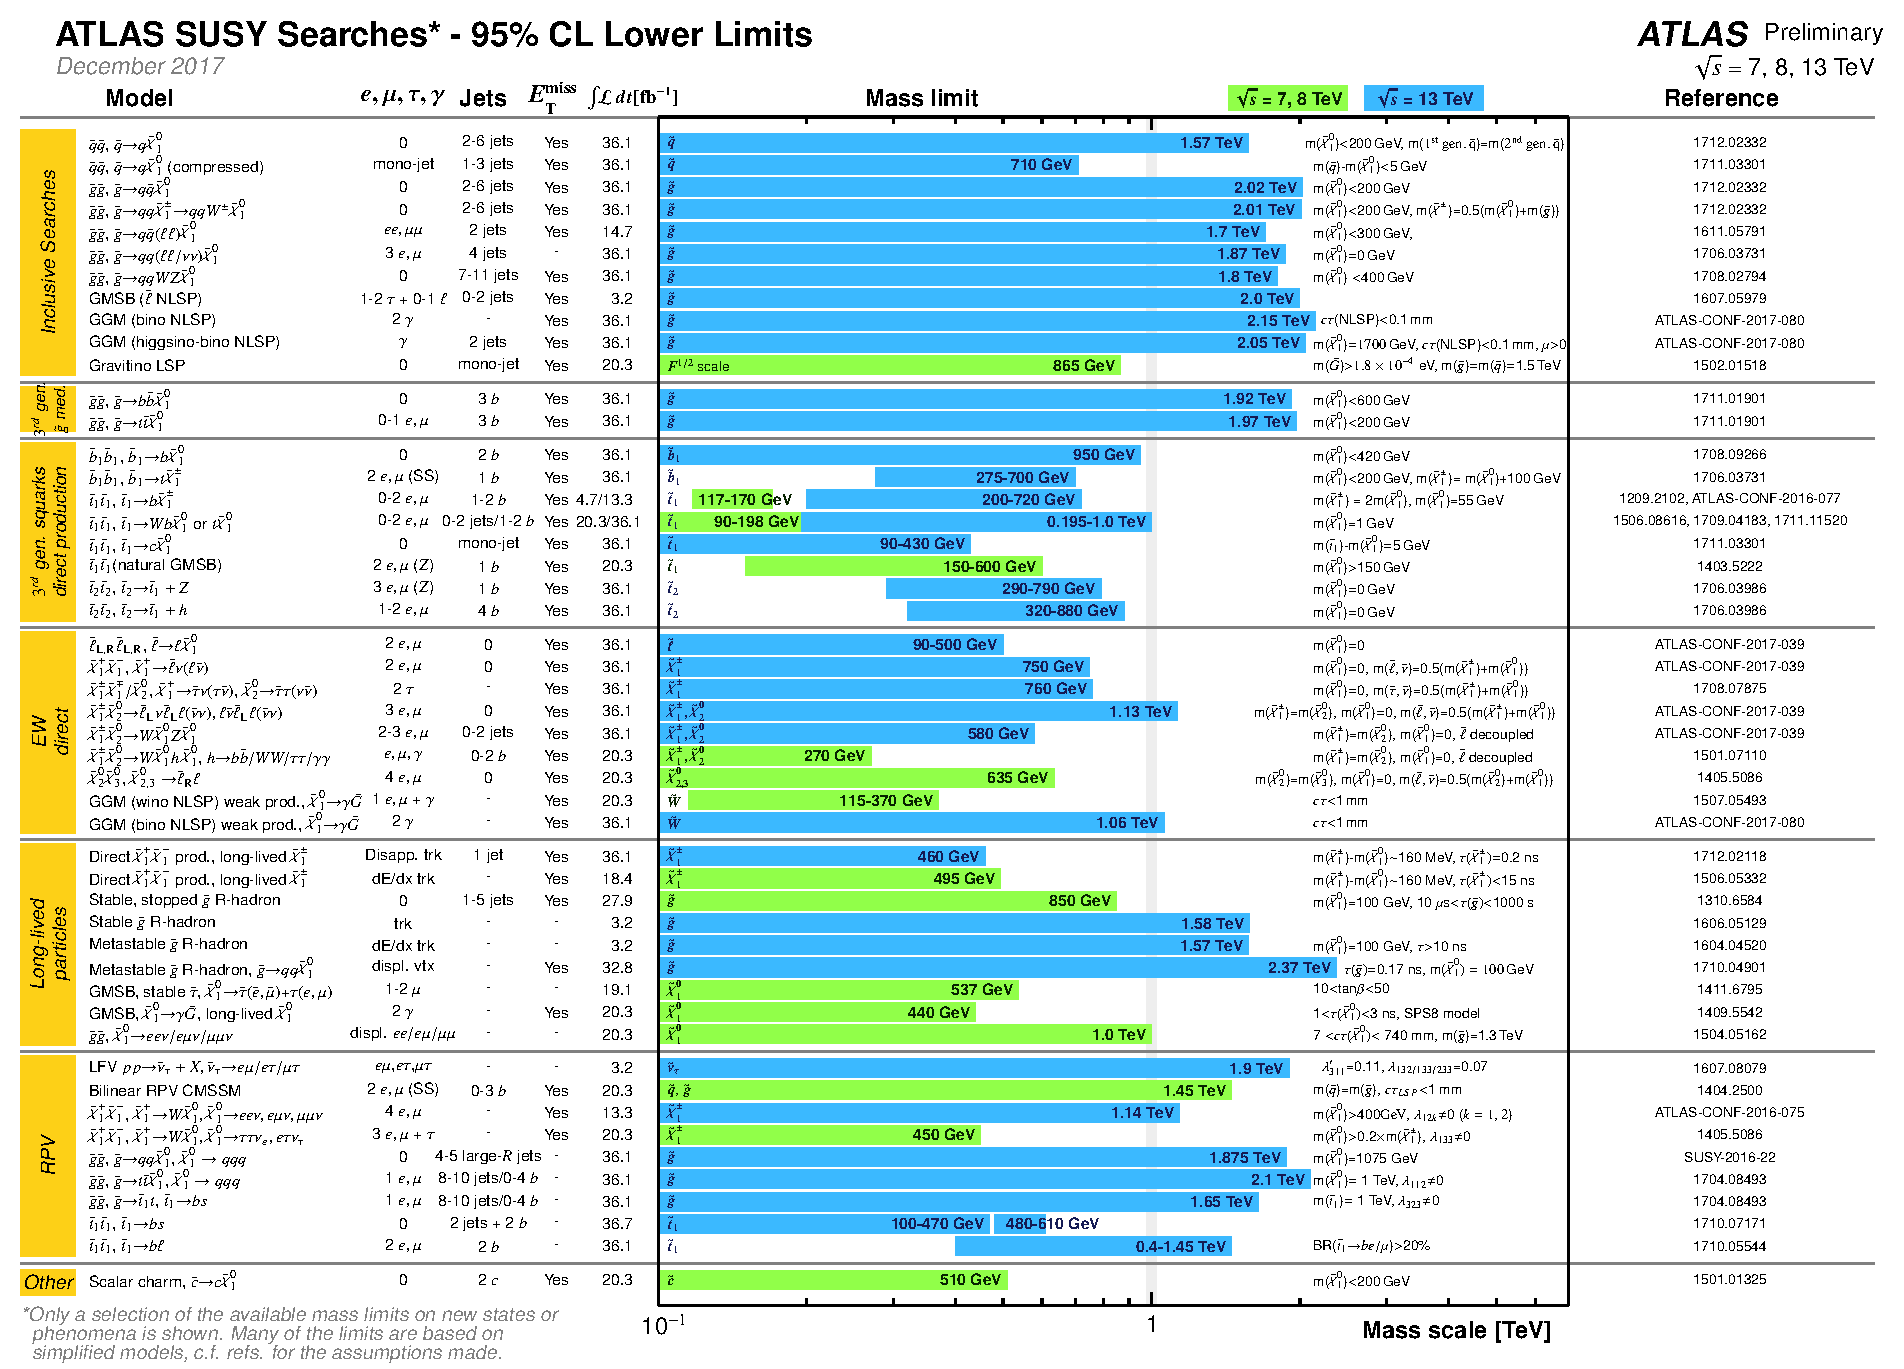
\includegraphics[width=\textwidth]{figures/ATLAS_SUSY_Summary.pdf}
\caption{Mass reach of ATLAS searches for a representative selection of results available in December 2017. From~\cite{ATLASSUSYSummary}.\label{fig:SUSYSummary}}
\end{figure}

No SUSY search so far has found evidence for the discovery of new particles, and the mass
reach of ATLAS searches using simplified models is shown in Fig.~\ref{fig:SUSYSummary}, with a similar reach for CMS searches. 
The lower limit on the masses of the strongly produced partners of quarks and gluons %for 100 GeV neutralino masses
are approaching 2 TeV (see e.g.~\cite{Aaboud:2017bac}). 
%picked the strongest gluino limit from https://atlas.web.cern.ch/Atlas/GROUPS/PHYSICS/CombinedSummaryPlots/SUSY/ATLAS_SUSY_Strong_all/ATLAS_SUSY_Strong_all.png
Heavy flavor supersymmetric partners are excluded below 1 TeV for light neutralinos (see e.g.~\cite{Sirunyan:2017wif}). %picked the latest stop 0L from CMS
Direct production of weakly coupled SUSY particles as LSP has a significantly lower production cross section with respect to strongly coupled SUSY partners,
and require larger integrated luminosities for discovery or exclusion, the combination of a variety of searches 
as in~\cite{Sirunyan:2018ubx} or specific signatures, e.g. requiring a highly energetic jet to the search
region to select events regardless of the low \MET from compressed spectra as in~\cite{Aaboud:2017leg} or
by exploiting the long lifetime arising from the small mass difference between the particles in the decay chain~\cite{ATL-PHYS-PUB-2017-019}. %CD: This is poor effort but do we want to give it more space? 
The searches for gauge boson superpartners (gauginos) have a reach of approximately 1 TeV if the superpartners
of SM leptons are light and the search can benefit from a high leptonic branching ratio, 
while the constraint on the gaugino masses reduces to 600 GeV if their decays proceed
through W and Z bosons.
%Maybe we shouldn't call them gauginos because that is more terminology? 

%Notes from the SUSY talk
%No evidence for Jet+MET SUSY (strong plain SUSY)
%Specifically target scenarios of gauge mediated: add photons to the final state and push sensitivity
%SUSY 2017 Gluino up to 2 TeV range. 
%There are parallels between the models
%Use exclusive combinations of objects
%Pick the right signal, very specific also in the mass spectrum 
%RPV: gravitino invisible particles 

%Higgsino searches nice to find projections for those. going to take a lot of luminosity.

%\subsubsection{pMSSM scans}

Targeting a specific signature, such as a cascade decay in a specific simplified SUSY model, 
drastically increases our ability to discover it. A narrower focus however trades generality for sensitivity. 
Designing and interpreting searches solely using simplified models may not capture the spectrum of possibilities
given by full, theoretically well motivated models. 

The concreteness of SUSY can be put to use to complement simplified models, by mapping search design and
interpretations to many different combinations of parameters in a full framework such as the pMSSM. 
Ref.\cite{Conley:2010du}, and continuing through LHC experiments ~\cite{Aad:2015baa, Khachatryan:2016nvf},
use the pMSSM to define a finite (though large) parameter space to probe. In this context, 
one can ask, systematically, what regions of the parameter space are already excluded by
existing results and what regions remain viable. 
%, and why those regions have so far remained untouched. %CD: unclear how you can tell this from SUSY scans?

Even the approach of these scans does not provide rigid or exhaustive exploration of the possibilities,
as even the pMSSM relies on simplifying assumptions, but these efforts can provide a coarse-grained
map determining signatures that remain unexplored by current searches.  
Adding assumptions relating the LSP to a thermal relic, one can further narrow the list of search
targets and key in on particular regions of parameter space for prioritized studies, see e.g. Ref.~\cite{Aaboud:2016wna}
in the case of electroweak SUSY. 
%CD: I would leave this discussion for the relic section later. Otherwise we can start with:
%These assumptions are of course not to be taken as more than a guiding principle... 

Tools such as Mastercode~\cite{Bagnaschi:2017tru} and GAMBIT~\cite{Athron:2017ard} can also be used to fit SUSY (and generic BSM)
model parameters to data and cosmological constraints. The outcome of these codes, often ran on supercomputers, 
is the likelihood for the viability of sets of parameters of a SUSY model given the available results from
from both searches at colliders as well as Standard Model precision measurements and direct and indirect Dark Matter detection experiments.

%CD: I am not 100% sure I can convey this in three lines.

%global fitting code for generic Beyond the Standard Model theories, designed to allow fast and easy definition of new models, observables, likelihoods, scanners and backend physics codes.
%code that allows to fit different versions of the Minimal Supersymmetric Standard Model (MSSM) to currently existing experimental data.


%(cite battaglia etc? and ATLAS paper with relic?). Mention that these assumptions are of course very tenuous,
%as they deal with physics at potentially much higher energy scales. But invisible particles density is one
%of the only clues we have about BSM, so more, not less, of this sort of thing is interesting to do (i.e. vary the assumptions).

%Other tools to do this. GAMBIT.

%Tools exist to approac

%\subsubsection{Models with long-lived particles}
%This serves as transition for the LLP chapter


\subsection{Searches for invisible particles in association with long-lived particles}
\label{sec:results_LLPSearches}

%TODO: polish transition from NLSP talk above (which e.g. could be metastable and long lived) to talking about the exotics/general counterpart to susy.
The experimental detection of the long-lived particles produced in association with the invisible particles candidates depends on their lifetime. 
In case of short lifetimes, the LLP will decay in the inner detector, giving rise to displaced vertices. Longer lifetimes will lead
to decays in the calorimeters or in the muon spectrometers. The detection of massive particles decaying outside the detector needs to rely
on their electromagnetic charge, using e.g. the distribution of energy released within the pixel detector ($dE/dx$) in association
with calorimeter timing so to have two independent detectors. Particles with even longer lifetimes can be detected in the empty bunch
crossings of the LHC. %Mathusla? or in future? https://arxiv.org/abs/1606.06298
Another distinctive experimental signature of LLP is the "disappearing track", produced for example by SUSY models where a chargino
%we haven't defined chargino i think
with a short lifetime leaves a track in the inner detector which effectively disappears as it decays into a neutralino and a soft pion. 
(1712.02118). 

%summary diagram in https://indico.cern.ch/event/656211/contributions/2673379/attachments/1498650/2333150/UW_dark_photons.pdf

The LHC searches mentioned in this chapter, with the exception of compressed SUSY scenarios, 
so far target prompt production of WIMP invisible particles or associated mediator particles at colliders. 
The absence of a signal constrains these traditional WIMP models to have small cross-sections and high mass scales. 
This is one of the reasons why less-accessible dark boson and dark scalar models, including mediators with masses from the MeV to the tens
of GeV and with a range of potential lifetimes, are a target that is gaining interest by LHC searches. A similar consideration
applies for SUSY scenarios that are hard to detect. 

%Split SUSY ATLAS: 1710.04901 


%The list of results
%below is only an example of LHC searches for dark photons to exemplify the upcoming opportunities for these signatures at colliders. 

These signatures are particularly challenging for ATLAS and CMS, given that many of these possibilities escape
conventional detection (e.g. decay outside the tracking volume, requiring custom reconstruction techniques, or 
are too light to be selected by the trigger). 
Collider experiments can still search for distinctive detector signatures from visible decays of light dark bosons. 
For example, the searches in~\cite{ATLAS:2016jza} look for \textit{lepton-jets}, collimated decay products of light,
long-lived boosted dark bosons.
%Prompt also exists, see Miriam's diagram
The BR of the SM Higgs boson is found to be below 10\% for a range of masses and lifetimes. This search benefits from tailored
trigger and reconstruction algorithms for collimated muons. Other examples of searches for dark photons at
general purpose experiments are exotic decays of the Higgs boson~\cite{Aad:2015sva.CMS-PAS-HIG-16-035}, 
where dark bosons are pair-produced and decay to muons. 
%The CMS mass range covered is 0.25-8.5 GeV, while the ATLAS range is 15 and 60 GeV
%Lepton-jets are also produced in SUSY cascade decays. 
%https://indico.cern.ch/event/492240/contributions/2302157/attachments/1367524/2072266/Leptonjets_HiggsCoupling_Nov2016_Safonov.pdf
%fun substructure for electron jets
%https://journals.aps.org/prd/abstract/10.1103/PhysRevD.95.055007
%If we want to mention sterile neutrinos (probably not), https://journals.aps.org/prd/abstract/10.1103/PhysRevD.91.093010
Drell-Yan dilepton production
and electroweak precision observables are also sensitive to these models~\cite{Curtin:2014cca},
due to the mixing of the dark boson with the SM bosons. 
%Mention sensitivity? See Shelton's talk
The LHCb experiment can exploit precise tracking 
to search for visible decays of both prompt and long-lived dark vector bosons into muon pairs~\cite{Aaij:2017rft},
providing the most stringent constraints on dark bosons between 10 and 70 GeV. Dimuon pairs are 
also exploited to search for dark scalar particles with a long lifetime~\cite{Aaij:2016qsm}. %Results:
%Lifetimes of: 2�10?10 and 10?7
%masses of: No significant excess is observed in the accessible ranges of mass 250<m(?)<4700MeV/c2 and lifetime 0.1<?(?)<1000ps. 
LHCb is a non-hermetic forward experiment so it needs to rely on visible decays of the dark particles. 
Experiments at electron-positron colliders, such as the BaBar and Belle experiments,
exploit the knowledge of the center-of-mass energy as a constraint to compensate their non-hermeticity, 
and set stringent collider limits on the kinetic coupling $\epsilon$ for this kind of models
for dark boson masses between 0.5 and 10 GeV. 


%%%%%%%%
%ASSORTED JUNK
%%%%%%%%

%beginning with the searches that illustrate many of the experimental 
%
%
% and then signals of MET. 
%
% description has a historical and ordering
%We begin with introducing 
%
%start with introducing the searches, mostly  
%
% of invisible particles searches, we will turn to a [categorization] of the searches done so far. After a summary of searches for interactions through SM bosons, we turn to the experimental results 


%As described in the previous chapter, invisible particles itself is not visible at colliders and has
%to be observed indirectly in association with other visible particles. 
%
%Signals of invisible particles can come from MonoX and diX searches. 
%
%State of the art MC:
%
%Vector and scalar models are known at NLO~\cite{Neubert:2015fka,Haisch:2013ata}
%NLO corrections for vector and scalar models in monoZ and monojet
%
%t-channel
%
%From Millie's talk (see Reaction OmniOutliner):
%Since the invisible particles-mediator-quark vertices allow for simultaneous FS partons with different hard scale, particular prescription needs to be used for the generation of samples with different partons that splits samples in number of mediators. Interference between the diagrams is neglected following Papucci et al. 